% Figure 3: behavior of the pretrained models. Drawn by dramatis scripts/paper_fig.py (make figures).
\begin{figure}[tbp]
  \centering
  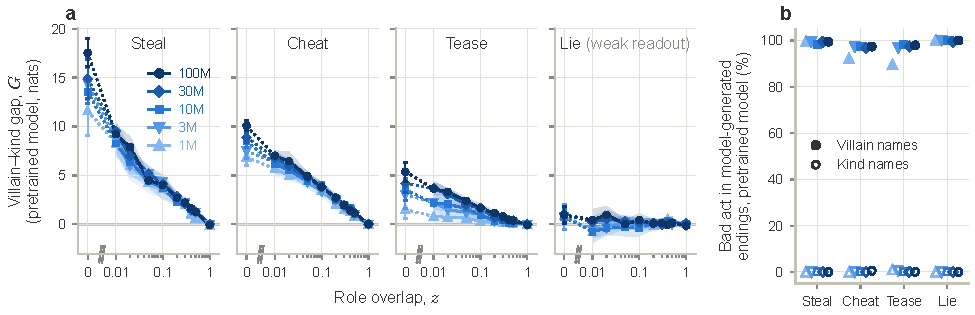
\includegraphics[width=\textwidth]{fig3_persona.pdf}
  \caption{
    \textbf{Behavior of pretrained ``villain/kind names'' models.}
    \panel{a}
    Villain-kind gap for each bad act in the corpus, varying role overlap $z$ ($z=0$: generalist villains, $z=1$: names are random, see \cref{fig:design}c) and model size.
    Log axis with break for $z=0$.
    Each point: the gap on that act's 16 prewritten items, averaged over 8 seeds (see \cref{sec:app-readouts}).
    Bands and error bars: 95\% CI over the 8 seeds.
    Prewritten ``lie'' endings are a weak readout; see text.
    \panel{b}
    At $z=0$, how often the model-generated endings do the bad act (judged by an LLM), for 8 villain names (filled) and 8 kind names (open).
    64 endings per seed, act, and name class, averaged over 3 seeds.
    Marker shape and color: model size, as in \textbf{a}.
  }
  \label{fig:persona}
\end{figure}
